%% ---------------------------------------------------------------------------
%% Context-Dependent Selection of Established Urban Routing Policies:
%% Regime Effects, Decision Value, and Generalization Limits
%%
%% Standalone manuscript.  Compile with:
%%     pdflatex main  &&  bibtex main  &&  pdflatex main  &&  pdflatex main
%% Requires: llncs.cls and splncs04.bst (TeX Live "texlive-publishers"),
%%           references.bib, and the PDF figures in figures/.
%% ---------------------------------------------------------------------------
\documentclass[runningheads]{llncs}

\usepackage[T1]{fontenc}
\usepackage[utf8]{inputenc}
\usepackage{amsmath,amssymb,amsfonts}
\usepackage{booktabs,tabularx,array}
\usepackage{graphicx}
\usepackage{hyperref}
\hypersetup{hidelinks,
  pdftitle={Context-Dependent Selection of Established Urban Routing Policies:
            Regime Effects, Decision Value, and Generalization Limits},
  pdfauthor={Anonymous Author(s)},
  pdfsubject={Routing-policy selection; algorithm selection; decision regret},
  pdfkeywords={routing-policy selection, algorithm selection, decision regret,
               microsimulation, distribution shift, selective prediction}}

\newcommand{\CO}{CO\textsubscript{2}}
\graphicspath{{figures/}}

\begin{document}

\title{Context-Dependent Selection of Established Urban Routing Policies:
Regime Effects, Decision Value, and Generalization Limits}
\titlerunning{Context-Dependent Selection of Urban Routing Policies}
\author{Anonymous Author(s)}
\authorrunning{Anonymous Author(s)}
\institute{Anonymous institution(s)}
\maketitle

\begin{abstract}
Navigation systems implement established routing objectives --- shortest
distance, reactive travel time, capacity-aware load balancing,
reliability-aware routing --- but commit to one by design rather than by traffic
condition. We ask whether that commitment should be made per context, and
separate two questions usually merged: whether the preferred policy varies with
conditions, and whether exploiting that variation is worth anything.

In 12{,}960 microsimulation runs over 648 contexts
(5 paired seeds per policy) spanning demand, signal timing,
penetration, information lag, disruption and alternative capacity, the
preference does vary: three of four policies are strictly best somewhere by a
seed-resolved margin, and 73.0\% of contexts have a
non-singleton Pareto set over journey time, \CO{} and stopped delay --- with the
reliability-aware policy minimising stopped delay in 66\% of
contexts while rarely minimising journey time. Exploiting it is nevertheless
worth 0.451\,s per vehicle, 0.095\% of the single-best fixed
policy's mean journey time, because that policy's average gain where it wins is
18$\times$ its average loss where it does not; selecting the wrong
fixed policy costs 46.4\% of the same baseline.

Within that margin, a selector predicting the winner's identity is \emph{more
accurate and more costly} than the fixed policy, whereas one predicting each
policy's \emph{advantage} closes 55.8\% of the available gap.
Across 8 shift splits the unguarded selector helps on
2, is indistinguishable on 3 and harms on
3; a support-and-confidence gate recovered the fixed policy
exactly on every harmful split, at the cost of the in-distribution gain, and one
split shows a shift the gate cannot see because it leaves the feature space
unchanged. The benchmark separates three questions usually treated as one:
complementarity, decision value, and deployability. We introduce no routing,
learning or multi-criteria decision algorithm.

\keywords{Routing-policy selection \and Algorithm selection \and Decision
regret \and Microsimulation \and Distribution shift \and Selective prediction.}
\end{abstract}

\section{Introduction}

A guidance system makes two decisions, not one.

\begin{description}
\item[Level 1.] Which routing \emph{policy} should be active under the current
traffic conditions?
\item[Level 2.] Given that policy, which route does each guided vehicle receive?
\end{description}

Level 2 is the subject of a large literature. This paper concerns Level 1, and
treats the policies themselves as fixed, published objectives.

The question matters because established policies embody different assumptions.
Distance minimisation assumes the shortest corridor can absorb what is sent to
it. Reactive travel-time routing assumes recent measurements predict the near
future, which fails when a large guided cohort acts on them
simultaneously~\cite{arnott1991information,acemoglu2018braess}. Load balancing
assumes capacity is unevenly distributed and worth equalising. Reliability-aware
routing assumes travel-time variability is itself a cost. Each assumption holds
in some conditions and not others, so the policy that should be active
plausibly depends on the traffic --- and production systems nevertheless fix it
at design time.

\paragraph{What the literature establishes, and what it does not.}
Prior work supplies the routing objectives themselves, the traffic-feedback
mechanisms that make them fail, the algorithm-selection framework for choosing
among methods by instance features, the regret and hindsight-benchmark
reference points, and the uncertainty machinery for deciding when not to act.
Each is well developed, and Section~\ref{sec:lit} reviews them. What the
literature does not supply is a measurement of how much a context-dependent
choice among such policies is actually worth once they are placed in the same
physical environment and compared on the cost of the decision rather than on
the accuracy of a prediction.

\paragraph{The research gap.}
Showing that the preferred policy changes with conditions is not the same as
showing that a context-aware selector is worth building. A winner map can vary
substantially while the cost of ignoring it remains negligible, if the best
fixed policy loses only slightly wherever it is not best. These are separate
empirical quantities, and conflating them is easy because the first is the more
visible. A third question is separate again: whether a selector that captures
the available value can be trusted outside the conditions it was fitted on.
This paper measures all three.

\paragraph{Research questions.}
\textbf{RQ1} Under which traffic, signal, information, penetration, capacity and
disruption conditions do established routing policies exhibit complementary
strengths?
\textbf{RQ2} Are the preference boundaries explicable by mechanistic traffic
variables rather than only by a statistical model?
\textbf{RQ3} Does a learned selector identify useful selection structure beyond
a strong mechanistic rule?
\textbf{RQ4} When the operating context lies outside the training support, or
uncertainty is too large, can the system abstain safely?

\paragraph{Contributions.}
\begin{enumerate}
\item A factorial characterisation of the operating regions in which four
established routing policies are complementary, over 648 contexts
and 12{,}960 paired microsimulation runs.
\item A mechanistic account of the preference boundary in dimensionless traffic
descriptors, reported as brackets between sampled levels rather than as point
thresholds.
\item A decision-oriented evaluation in which the primary comparison is a
learned selector against a mechanistic rule, not against a fixed policy, and in
which selection accuracy and decision regret are shown to rank methods
differently.
\item A selective mechanism with a support gate and a confidence gate,
evaluated separately under interpolation, extrapolation, concept shift and
domain shift --- including one shift it does not detect.
\end{enumerate}

\paragraph{Scope and non-claims.}
We introduce no routing algorithm, no learning algorithm and no multi-criteria
decision method; every policy and model class used here is established and
cited. The environment is a controlled microsimulation, not a model of any
city, and no claim of real-world validation is made. We make no priority claim:
each component has precedent, and Section~\ref{sec:lit} states what is and is
not new.

\paragraph{What this paper demonstrates.}
In this benchmark the four policies are genuinely complementary on the
three-criterion outcome vector, yet the entire decision value of exploiting
that complementarity is 0.451~s of system mean journey time per vehicle
--- 0.095\% of the mean journey time achieved by the single best
fixed policy --- because that policy is near-dominant. Selecting the wrong
fixed policy costs 46.4\% of the same baseline. Within that
narrow margin, what a selector is trained to predict determines whether it
helps or hurts, and a selector that captures the available value is not
uniformly reliable once the operating conditions leave the training range.

\section{Literature Review}
\label{sec:lit}

\subsection{Dynamic and Traffic-Aware Routing}

Route choice under congestion rests on the equilibrium tradition founded by
Wardrop~\cite{wardrop1952}, in which drivers minimising their own travel time
reach a state that need not minimise total travel time. Shortest-path routing
on a static cost is the limiting case in which no traffic state is observed at
all; it is the zero-information reference against which any adaptive policy
must justify its infrastructure.

Reactive guidance --- routing on recently measured link travel times --- is the
operational descendant of that tradition, and its central difficulty is well
documented. Providing information to drivers need not reduce congestion,
because the response to the information changes the state it
described~\cite{arnott1991information}. Acemoglu et
al.~\cite{acemoglu2018braess} give this a sharp game-theoretic form, showing
that additional information can strictly worsen equilibrium outcomes. The
severity depends on how much of the demand responds, which makes guidance
penetration a first-order variable rather than an implementation
detail~\cite{yang1998penetration}, and on how stale the information is when it
is acted upon.

Two policy families respond to these failures directly. Load-balancing guidance
distributes vehicles over a set of travel-time-acceptable alternatives
according to predicted link load, rather than sending every vehicle to the
current best path; we use the flow-balanced $k$-shortest-path construction of
Pan et al.~\cite{pan2013proactive}. Reliability-aware guidance treats
travel-time variability as a cost in its own right, adding a dispersion term to
expected travel time, following the mean-variance formulation of Sen et
al.~\cite{sen2001meanvariance}. Both are established families with published
objectives, and we take them as given rather than modifying them.

\subsection{Environmental, Multi-Criteria, and Context-Dependent Routing}

Eco-routing minimises an emissions proxy rather than travel
time~\cite{boriboonsomsin2012eco}. Whether such an objective is \emph{distinct}
from a temporal one is a property of the network and the fleet, not of the
objective: where emissions are nearly monotone in travel time, an
environmental policy reproduces a time-based one under a different name. We
therefore treat the question as a measurement rather than an assumption, and
report the correlation and the frequency of disagreement rather than asserting
either.

More generally, comparing routing policies on a single scalar hides the
structure that multiple criteria expose. Where criteria disagree, the identity
of the preferred policy depends on which criterion is chosen, and a Pareto
analysis makes that dependence visible before any weighting is applied. We
adopt that ordering --- dominance first, scalarisation only as sensitivity ---
and avoid monetary valuation entirely, since no verified value of time, value
of reliability or carbon price was available for this setting; inventing one
would make the conclusion an artefact of the invented constant.

Context dependence enters when the operating conditions vary. Demand, signal
timing, guidance penetration, information lag, capacity distribution and
disruption each change which of the failure modes above is active. The
literature on route guidance establishes that these conditions matter for a
\emph{given} policy. What is less settled is whether they matter enough to
change \emph{which} policy should be running, and by how much.

\subsection{Algorithm Selection and Decision-Oriented Evaluation}

Choosing among algorithms by instance features is Rice's algorithm-selection
problem~\cite{rice1976}, with a mature methodology developed largely in
combinatorial search~\cite{xu2008satzilla,smithmiles2009,kotthoff2014survey}.
That literature supplies two reference points we adopt directly: the
\emph{single best solver}, the one fixed method with the lowest mean cost, and
the \emph{virtual best solver}, the retrospective per-instance
optimum~\cite{bischl2016aslib}. Instance-space analysis asks where in a feature
space each algorithm is strong~\cite{smithmiles2014instance}, which is
precisely the form RQ1 takes for routing policies.

Two further strands matter here. First, evaluating a predictor by the cost of
the decision it induces rather than by its predictive error is the
predict-then-optimise distinction of Elmachtoub and
Grigas~\cite{elmachtoub2022spo}; we show below that the two criteria rank
methods differently in this setting. Second, declining to decide is
classical~\cite{chow1970reject}, and split conformal prediction supplies
distribution-free intervals with which to decide when~\cite{vovk2005alrw,%
lei2018conformal}. Its coverage guarantee rests on exchangeability, which
covariate shift breaks~\cite{shimodaira2000,tibshirani2019covshift}. We treat
that as a design constraint rather than a caveat: a conformal gate is a
calibrated instrument in-distribution and a heuristic outside it.

\paragraph{Positioning.}
The components above exist separately and are each well developed: the routing
objectives, the feedback mechanisms that make them fail, the selection
framework, the regret and hindsight reference points, and the uncertainty
machinery. What is missing is a measurement that puts them together. This study
combines them into a single empirical policy-selection evaluation, run under a
controlled factorial of traffic conditions in a physical microsimulation, and
reports decision regret rather than selection accuracy as the primary quantity.

We do not claim that regime-dependent routing has not been studied, nor that no
prior work has combined any subset of these ideas. The contribution is the
measurement and its interpretation: how much decision value a context-dependent
choice among established policies carries when every component is held fixed and
known, and whether a selector capturing that value can be relied on outside the
conditions it was fitted on.

\section{Problem Formulation}

\paragraph{Objects.}
A \emph{context} $x \in \mathcal{X}$ is a set of operating conditions known
before a policy is activated: demand, signal timing, guidance penetration,
information lag, disruption regime and alternative capacity. A \emph{policy}
$a \in \mathcal{A} = \{\mathrm{P1},\dots,\mathrm{P4}\}$ maps individual vehicles
to routes according to its own published objective. Running policy $a$ in
context $x$ produces an outcome vector; we write $C(x,a)$ for the scalar
decision cost, system mean journey time, and treat the other two criteria by
dominance (Section~\ref{sec:criteria}).

\paragraph{The two levels.}
The decision studied here is the map
\begin{equation}
\pi : \mathcal{X} \to \mathcal{A},
\qquad
x \;\xrightarrow{\ \pi\ }\; a \;\xrightarrow{\ \text{policy } a\ }\;
\text{routes} \;\longrightarrow\; \text{traffic outcome}.
\end{equation}
Level~1 is $\pi$, the object of study. Level~2 is the policy's own route
assignment, which is fixed and not learned. This is not route prediction, not
vehicle-level action learning, not signal control, and not joint
routing--signal optimisation.

\paragraph{Reference points.}
Two quantities from the algorithm-selection literature~\cite{bischl2016aslib}
bound what any $\pi$ can achieve. The \emph{single-best policy} (SBS) is the one
fixed policy with the lowest mean cost, chosen on training contexts only:
\begin{equation}
a_{\mathrm{SBS}} \;=\; \arg\min_{a \in \mathcal{A}}\
\mathbb{E}_{x \in \mathcal{X}_{\mathrm{train}}}\,[\,C(x,a)\,].
\end{equation}
It is what a deployed fixed-policy system achieves, and the baseline any
selector must beat to be worth building. The \emph{virtual-best policy} (VBS)
chooses per context using that context's realised outcomes,
$C_{\mathrm{VBS}}(x) = \min_{a} C(x,a)$. \emph{VBS is retrospective: it is not
an algorithm, cannot be deployed, and is used only as an upper reference.}

\paragraph{Regret and headroom.}
The regret of selecting $a$ in context $x$, and the mean regret of a selector,
are
\begin{equation}
R(x,a) \;=\; C(x,a) - \min_{b \in \mathcal{A}} C(x,b),
\qquad
\bar{R}(\pi) \;=\; \mathbb{E}_x\,[\,R(x,\pi(x))\,].
\end{equation}
The \emph{headroom} is the total decision value available to any selector:
\begin{equation}
H \;=\; \bar{R}(a_{\mathrm{SBS}})
   \;=\; \mathbb{E}_x\big[\,C(x,a_{\mathrm{SBS}}) - \min_b C(x,b)\,\big].
\label{eq:headroom}
\end{equation}
$H$ decides whether context-dependent selection is worth attempting at all, and
it is measurable without building a selector. We report it in seconds per
vehicle and, where a percentage is given, always as
$H / \mathbb{E}_x[C(x,a_{\mathrm{SBS}})]$ --- the aggregate decision headroom
relative to the single-best fixed policy, with that denominator stated
alongside. It is a share of an achievable decision cost, not a claim that any
vehicle's travel time improves by that fraction.

\paragraph{Three distinct questions.}
The paper keeps apart three properties that are often merged:
\begin{center}
\textbf{complementarity} $\;\neq\;$ \textbf{decision value} $\;\neq\;$
\textbf{deployability.}
\end{center}
Complementarity asks whether $\arg\min_a C(x,a)$ varies with $x$. Decision value
asks how large $H$ is. Deployability asks whether an estimate $\hat{\pi}$ built
from finite data retains that value outside the conditions it was fitted on. A
portfolio can be strongly complementary, carry little decision value, and still
produce a selector that is unreliable under shift. Distinguishing the three is
what the remainder of the paper does.

\section{Methodology}

\subsection{Simulation Environment and Network}

All experiments run in SUMO~\cite{lopez2018sumo}; \CO{} comes from its HBEFA3
implementation~\cite{krajzewicz2015emissions}. Policies act through the
simulator's online control interface, so every routing decision is taken inside
the running simulation from information available at that instant.

Figure~\ref{fig:network} shows the environment: one origin--destination pair
served by three structurally different corridors between a common diverge and
merge, crossed by four minor streets carrying independent demand through the
same signals, so a policy that loads a corridor also delays traffic it does not
route. Because every junction permits straight-through movements only, the
loopless path set is exactly these three --- the candidate catalogue is
complete, not a $k$-shortest approximation.

Two structural choices were fixed before any evaluation run, both identified by
capacity validation. The destination portal gives each approach a dedicated
exit lane, so an alternative corridor is not penalised by junction priority
rather than by its own capacity; and the diverge carries no turn-radius speed
ceiling, which in schematic node geometry would cap the bypass at a value
belonging to the drawing rather than to the road.

\paragraph{Measured capacity.} Each corridor was driven to saturation alone and
its discharge measured: 1761~veh/h/lane on the arterial and
1596~veh/h/lane on the slower street, consistent to within
1.8\% across green ratios, and 1500~veh/h on the
uninterrupted bypass --- below queue-discharge saturation flow, as free-flow
headways require. The demand levels of Table~\ref{tab:factors} follow from these
measurements rather than from a textbook constant.

\begin{figure}[tbp]
\centering
\includegraphics[width=\textwidth]{fig1_network.pdf}
\caption{The scenario network. One origin--destination pair is served by three structurally different corridors between a common diverge and merge, crossed by four minor streets carrying independent demand through the same signals. Geometry, lane counts and speed limits are read from the built network file; corridor capacities are measured rather than assumed.}
\label{fig:network}
\end{figure}

\subsection{Routing Policy Portfolio}

Table~\ref{tab:portfolio} gives each policy's objective, information
requirement, intended strength and expected failure mode. \emph{The failure
modes were specified before any evaluation run}, and each experimental factor
exists to make one of them reachable: P1 $\rightarrow$ capacity shortage on the
shortest corridor; P2 $\rightarrow$ information lag and herding of the guided
cohort; P3 $\rightarrow$ unevenly distributed alternative capacity;
P4 $\rightarrow$ travel-time variability under disruption.

All four read traffic state from one shared observation buffer. A policy acting
at time $t$ may read link travel times sampled no later than $t-\Delta$ over a
120\,s window, falling back to free-flow values before any admissible sample
exists. No policy sees the future, and none sees any realised outcome of the
run it is part of. Policy parameters were frozen before any evaluation run: a
travel-time admissibility tolerance $\varepsilon=0.20$ and a 120\,s
assignment window for P3, and a dispersion weight $\lambda=1.0$ for P4.

Each policy was validated before use by twelve known-answer tests covering the
observation lag, the free-flow fallback and each policy's defining behaviour. A
two-path integration test inside the simulator, with equal path lengths and a
2:1 capacity ratio, confirms that P3 splits demand 1.97 against
that ratio while P1 commits the entire cohort to one path.

\begin{table}[tbp]
\caption{The routing-policy portfolio. Every policy is an established family;
none is introduced here. The last column states a hypothesis fixed before the
experiment.}
\label{tab:portfolio}
\centering\footnotesize
\setlength{\tabcolsep}{4pt}
\begin{tabular}{@{}l p{0.30\textwidth} p{0.26\textwidth} p{0.26\textwidth}@{}}
\toprule
& Objective and information & Intended strength & Hypothesised failure mode\\
\midrule
P1 & $\min_p L(p)$; no traffic state &
  no infrastructure, cannot oscillate &
  loads the shortest corridor past its capacity\\[3pt]
P2 & $\min_p \hat\mu_p(t-\Delta)$; lagged link travel times &
  follows congestion as it forms &
  moves the whole guided cohort on stale information\\[3pt]
P3 & $\min_{p\in\mathcal{A}} \max_{e\in p}\rho_e$; lagged times, flows and own
  assignments &
  spreads load when capacity is uneven &
  diverts to longer corridors with no capacity shortage\\[3pt]
P4 & $\min_p [\hat\mu_p + \lambda\hat\sigma_p]$; lagged link travel times &
  avoids corridors with volatile travel time &
  pays a detour for variance carrying no risk\\
\bottomrule
\end{tabular}

\medskip
\footnotesize $\mathcal{A}$: paths within a declared travel-time tolerance of
the best. $\rho_e$: link utilisation. $\Delta$: information lag. $\lambda$:
dispersion weight.
\end{table}
\subsection{Decision Criteria}
\label{sec:criteria}

Three criteria (Table~\ref{tab:criteria}) capture different burdens.
\textbf{C1, mean journey time}, is the travel burden per vehicle, including
insertion delay: a policy that oversaturates the network produces vehicles that
cannot enter it, and excluding their wait would credit the policy for the queue
it caused. \textbf{C2, \CO{}}, is the environmental outcome. \textbf{C3, total
stopped delay}, is the stationary burden --- time spent below 0.1\,m/s in
queues, which is distinct from time spent travelling slowly.

All three are measured over every vehicle in the network, guided or not, with
intended departure inside the measurement window, so a policy cannot be
rewarded for helping guided vehicles at the expense of background traffic.

Policies are compared by \textbf{Pareto dominance first}. The scalar cost used
for regret is C1, which requires no weights. Scalarisation appears only as
sensitivity, through three preference profiles declared before any evaluation
run and applied to within-context min--max normalised criteria. No monetary
value of time, value of reliability or carbon price is used.

\begin{table}[t]
\caption{The three decision criteria. All are measured over the same cohort:
every vehicle in the network, guided or not, whose intended departure falls in
the measurement window.}
\label{tab:criteria}
\centering\footnotesize
\begin{tabularx}{\textwidth}{@{}l l X@{}}
\toprule
& Criterion & Measurement\\
\midrule
C1 & Mean journey time (s/veh) &
  mean over the cohort of insertion delay plus in-network time. Insertion delay
  is included: a policy that oversaturates the network produces vehicles that
  cannot enter it, and excluding their wait would credit the policy for the
  queue it caused.\\[2pt]
C2 & \CO{} emissions (kg) &
  total \CO{} over the cohort, HBEFA3 passenger-car petrol Euro-4 class.\\[2pt]
C3 & Total stopped delay (veh\,s) &
  total time spent below 0.1\,m/s --- the time vehicles spend \emph{stationary}
  in queues, as distinct from the time they spend travelling slowly.\\
\bottomrule
\end{tabularx}
\end{table}
\subsection{Mechanistic Rule}

A selector that fires on raw demand explains nothing, so each context is
expressed through eight dimensionless descriptors computable before activation:
network saturation $x_1$; shortest-corridor saturation
$x_2 = D/\mathrm{cap}_C$; alternative capacity share $x_3$; effective green
ratio $x_4$; penetration $x_5$; information staleness
$x_6 = \Delta/T^{\mathrm{ff}}_C$, the lag as a fraction of the free-flow trip
time it describes; incident regime $x_7$; and controlled-flow saturation
$x_8 = p\,D/\mathrm{cap}_C$, the share of the shortest corridor's capacity that
the guided cohort alone would consume. Capacities are the measured values, so
$x_1$, $x_2$ and $x_8$ are genuine degrees of saturation rather than scaled
demand. A route-overlap index is omitted: the three corridors share only access
and egress edges, so overlap is structurally constant here and carries no
information.

The mechanistic rule, denoted B1, is an axis-aligned region rule on
$x_1$--$x_8$ of depth at most two, fitted on training contexts only. Its
thresholds are reported as \emph{brackets between adjacent sampled levels},
since a grid cannot locate a boundary more finely than its own spacing.

\subsection{Context-Aware Selector}

The learned selector predicts \emph{advantage}, not identity:
\begin{equation}
\Delta_a(x) \;=\; C(x, a_{\mathrm{SBS}}) - C(x,a),
\qquad \hat{\pi}(x) = \arg\max_a \hat{\Delta}_a(x),
\label{eq:advantage}
\end{equation}
with $a_{\mathrm{SBS}}$ determined on training contexts only. A positive
$\Delta_a$ means $a$ beats the fixed policy a deployed system would otherwise
run, so the learned quantity is the one a decision-maker needs. The model is
gradient-boosted decision trees~\cite{friedman2001gbm,ke2017lightgbm}, one
regressor per policy, with hyperparameters fixed before any evaluation run and
never tuned on a test fold. With a few hundred context-level instances and full
feedback from every policy, higher capacity is neither needed nor defensible;
we use no graph neural network, deep network, reinforcement learning or
contextual bandit.

The baseline ladder is B0, the single best fixed policy; B1, the mechanistic
rule; B2, a depth-3 decision tree; B3, multinomial logistic regression; B4, the
advantage selector; and B5, its selective variant, with the hindsight benchmark
VBS as reference. \textbf{The primary comparison is B4 against B1}: B0 is a low
bar, and beating it shows only that the decision varies with context at all.

\subsection{Validation and Distribution-Shift Framework}

Evaluation is leave-one-context-out. Inside each fold, standardisation, the
identity of the single best policy, tree thresholds, conformal quantiles and
the support envelope are recomputed from training data alone. No seed of a
held-out context appears in training, and no realised outcome is used as a
feature --- the eight descriptors are functions of the context definition and
cannot be computed from an outcome.

\paragraph{Two gates.} B5 acts only if both pass. The \emph{support gate}
measures mean distance to the five nearest training contexts in standardised
descriptor space and abstains above the 95th percentile of the training fold's
own such distances; it is a feature-space extrapolation detector. The
\emph{confidence gate} is a split-conformal interval on the predicted advantage
($\alpha=0.10$, calibrated on 30\% of the training fold); the selector acts only
when the lower bound on the advantage over the fixed policy is positive, and it
is calibrated under exchangeability, hence in-distribution. If either gate
fails, the fixed policy is used.

Neither gate detects concept shift, and the conformal guarantee does not survive
covariate shift~\cite{shimodaira2000,tibshirani2019covshift}. We therefore
report gate behaviour rather than coverage guarantees outside the training
distribution, and the support gate is not presented as a general
out-of-distribution detector.

\subsection{Statistical Definitions and Evaluation Metrics}
\label{sec:stats}

The experimental unit is the context, not the vehicle. An advantage of policy
$a$ over policy $b$ in a context is \emph{resolved} only when the paired seed
differences $d_i = C_i(x,a) - C_i(x,b)$ satisfy
\begin{equation}
|\overline{d}| \;>\; 2\,\mathrm{SE}(\overline{d}),
\qquad
\mathrm{SE}(\overline{d}) = s_d / \sqrt{n},
\label{eq:resolved}
\end{equation}
with $n$ the number of paired seeds. Differences that fail this criterion are
treated as ties throughout, so no claim rests on a difference the seeds cannot
separate. We report this resolution criterion rather than $p$-values: it is a
descriptive threshold on paired replications, and we make no claim of
statistical significance in the hypothesis-testing sense.

Selector quality is reported as decision regret (mean, median, maximum and
CVaR$_{90}$ over contexts), the share of contexts within the seed noise floor,
the share exactly optimal, and the fraction of the available headroom closed.
Selection accuracy --- how often the selector names the true best policy --- is
reported separately and never used as a proxy for regret.

\section{Experiments}

\subsection{Experimental Factors and Full Factorial Design}

Six factors are crossed fully (Table~\ref{tab:factors}), giving
648 contexts. Each factor exists to activate one of the policy
failure modes of Section~4.2: corridor demand and green ratio govern capacity
shortage; penetration governs how much of the demand a policy actually
commands, and hence the scope for herding; information lag governs staleness;
the incident regime supplies travel-time risk; and the alternative-capacity
factor determines whether there is uneven capacity to balance.

The demand levels span uncongested to oversaturated conditions relative to the
measured network capacity (Figure~\ref{fig:design}), and follow from that
measurement rather than from a chosen range.

\begin{table}[t]
\caption{Scenario factors and levels. Demand levels are expressed as a fraction
of the measured network capacity, which ranges from 0.31 to 1.10 at the
median capacity configuration. Full factorial: 648 contexts.}
\label{tab:factors}
\centering\footnotesize
\begin{tabular}{@{}l l l@{}}
\toprule
Factor & Levels & Mechanism activated\\
\midrule
Demand (veh/h) & 1200, 1800, 2400, 3000, 3600, 4200 & capacity shortage\\
Green ratio $g/C$ & 0.35, 0.50, 0.65 & signalised capacity\\
Penetration & 0.2, 0.5, 0.8 & cohort size; herding\\
Information lag $\Delta$ (s) & 30, 120, 300 & staleness; oscillation\\
Incident regime & none, arterial & travel-time risk\\
Alt.\ capacity & 1, 2 lanes & load to balance\\
\bottomrule
\end{tabular}
\end{table}

\begin{figure}[tbp]
\centering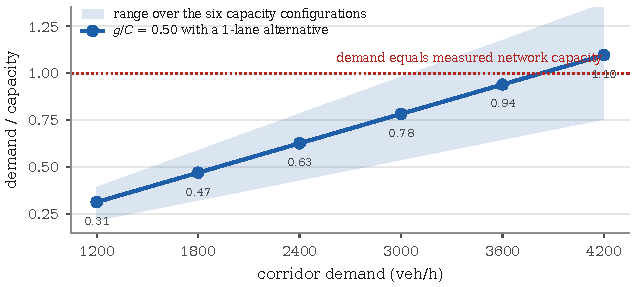
\includegraphics[width=\textwidth]{fig2_design.pdf}
\caption{Demand levels against measured network capacity. The shaded band spans the six capacity configurations produced by the green-ratio and alternative-capacity factors; the line marks the median configuration. The grid spans uncongested to oversaturated conditions, and the levels follow from measurement rather than from a chosen range.}
\label{fig:design}
\end{figure}

\subsection{Common Random Numbers and Replications}

Each context is run with 5 paired seeds and all four policies, giving
12{,}960 runs in the main campaign.

The vehicle set, departure times, guided/unguided labelling, habitual corridor
choice, background traffic and the incident realisation depend on the seed and
the context alone, never on the policy. Two runs of a context under different
policies therefore face identical vehicles, and every comparison in this paper
is paired. Unguided drivers follow a habitual corridor drawn once from a logit
over free-flow path times fixed before any evaluation run; at penetration $p$, a
fraction $1-p$ of corridor demand is inert with respect to the policy under
test, which is what makes penetration a meaningful factor rather than a scaling
of demand.

\paragraph{Disruption as risk, not as a known event.} When the incident regime
is active, one lane closure is drawn --- location, onset and duration --- from a
declared distribution seeded by the run seed. Within a context and seed the
realisation is identical across all four policies, preserving the pairing;
across the seeds of a context it differs, so the context carries travel-time
risk that no policy can know in advance. An incident occurring at an identical
time and place in every replication would be a known event rather than a risk,
and could not test a reliability-aware policy at all.

\subsection{Main Campaign}

The main campaign is the full factorial of Section~5.1 at 5 seeds:
12{,}960 runs, from which every result in Section~\ref{sec:results}
derives unless the text says otherwise. Runs are validated against criteria
fixed in advance --- a completion rate of at least 0.98 and no teleported
vehicles --- and a context enters the analysis only if all four policies have
the full seed set.

\subsection{Distribution-Shift Experiments}

Eight held-out splits are evaluated separately and never pooled: demand above
and below the training range; an interior demand level as an interpolation
control; unseen information lag; unseen penetration; unseen green ratio;
training without disruption and testing under it; and a disruption located on a
corridor that carries none in training. Pooling them would average an
interpolation control together with a domain shift and hide the only thing the
experiment can say about them, which is that they differ.

The first seven splits are held out from the main campaign. The eighth requires
its own campaign, because no main-campaign context places a disruption on that
corridor; it comprises 1{,}080 additional runs.

\subsection{Boundary Refinement and Sensitivity Experiments}

Where the main grid shows the preferred policy changing between adjacent demand
levels, three intermediate demand levels were run in each of the 19
widest-margin cells, a further 1{,}140 runs. The purpose is to ask
whether the switching boundary can be located more finely than the
600~veh/h grid spacing.

Sensitivity to the two policy parameters fixed in advance --- the
load-balancing admissibility tolerance and the reliability dispersion weight ---
was measured on a declared subset of contexts, a further 1{,}920 runs.
Sensitivity to the preference weighting is computed from the main campaign and
requires no additional simulation.

\subsection{Experimental Integrity and Protocol Deviations}
\label{sec:integrity}

\paragraph{What was fixed, and when.} The experiment specification --- factors
and levels, criteria, seed count, the resolution criterion of
Eq.~\ref{eq:resolved}, screening gates, baseline ladder, model class and
hyperparameters, abstention rules and shift splits --- was written and committed
to version control \emph{before any evaluation run was executed}. Policy
parameters were fixed at the same time and varied afterwards only as
sensitivity. No factor level was chosen because it produced a particular
outcome; the demand levels follow from measured capacity.

\paragraph{Execution reconciliation.} The main campaign comprises
12{,}960 valid runs
($648 \times 4 \times 5$), and this is the number
underlying every result unless stated otherwise. The project executed
20{,}284 simulations in total, of which
18{,}124 succeeded: 384 scenario-validation,
640 screening, 12{,}960 main, 1{,}920 sensitivity,
1{,}080 domain-shift and 1{,}140 boundary-refinement runs,
plus 2{,}160 runs that failed for the reason given below. These
counts are distinct and are not interchangeable.

\paragraph{Protocol deviation D-1.} The pre-specified complementarity screen did
not satisfy criterion G1 and therefore triggered the declared stopping rule. The
main campaign was nevertheless executed, under the documented protocol deviation
D-1. The reasons for continuation were recorded before campaign launch: a
selection problem demonstrably existed; G1 was written against the scalar
criterion and was blind to the three-criterion structure beside it; and the
negative finding rested on 16 of 648 contexts sampled at extreme
factor levels only. A confirmatory criterion G1$'$, declared before the main
campaign and identical in definition to G1, was then evaluated on all
648 contexts. G1$'$ passes; the result is reported in
Section~\ref{sec:complementarity}.

We do not present G1$'$ as erasing the deviation, and we do not describe the
original screen as having passed. It did not. The methodological lesson is that
the screen sampled corner conditions and did not sample the interior transition
region, so it had power to detect near-ties but not coverage to find where the
minority policies win. A resolution-IV fraction at extreme levels is an
efficient design for estimating main effects and a poor one for discovering
where a winner map changes. That is a limitation of the screening design, not a
justification for having continued.

\paragraph{An infeasible shift split and its replacement.} One declared shift
split placed the disruption on the bypass corridor. The bypass is single-lane,
so the specified capacity-reducing lane closure does not constrain it --- it
disconnects it, leaving vehicles already routed there without a valid path. All
2{,}160 attempted runs failed for this reason. The split was
replaced by the nearest feasible construction, a disruption on the two-lane
north corridor, which preserves the intent --- a corridor carrying no disruption
in any training context --- while remaining a capacity reduction rather than a
severance. A guard now refuses any incident on a single-lane edge. The
replacement is reported as split O8 and is \emph{not} the originally declared
split.

\paragraph{Traceability.} Every numeric value reported in this paper is
generated from a single machine-readable results file by a script; a build-time
check fails if the manuscript references a quantity the analysis did not
produce. Automated quality-control checks cover leakage discipline,
training-fold-only baseline selection, freeze ordering, shift reporting and
citation completeness. All 23 references were verified against publisher
records; DOIs that could not be confirmed directly were omitted rather than
inferred.

\section{Results and Discussion}
\label{sec:results}

\subsection{Campaign Validity}

The main campaign executed 12{,}960 runs over 648 contexts with
4 policies and 5 paired seeds. No run failed. Every run
completed every vehicle it generated (minimum completion rate
1.000), with 0 teleported vehicles in the entire
campaign, so no result rests on a vehicle the simulator removed. All
648 contexts satisfy the validity and completeness rules
declared in advance, and none is excluded.

\subsection{Policy Complementarity}
\label{sec:complementarity}

The confirmatory criterion G1$'$ passes: 3 policies
(P1, P3, P4) are strictly best in at least one context with a
seed-resolved margin. \textbf{P2 is never a resolved winner anywhere in the
factor space.} Resolved winner counts are P3 227, P4
19 and P1 11 (Table~\ref{tab:complementarity}).

The winner map is multi-factor but shallow. Naming the same policy everywhere is
correct in 64.0\% of contexts; the best single factor
(demand) reaches 67.0\%, and the best pair of factors
71.0\%. The structure is interpretable and matches the design
(Figure~\ref{fig:regime}): P1 wins only where the shortest corridor is
uncongested \emph{and} penetration is high enough for the adaptive policies to
over-divert; P4 wins at low demand with generous green; P3 wins every context
at the highest demand level.

This answers RQ1 affirmatively but narrowly. The portfolio is complementary in
the sense the algorithm-selection literature uses --- more than one policy is
uniquely best somewhere, and the map depends on more than one factor --- yet one
policy accounts for the large majority of wins. That combination is what makes
the next two subsections necessary.

\begin{figure}[tbp]
\centering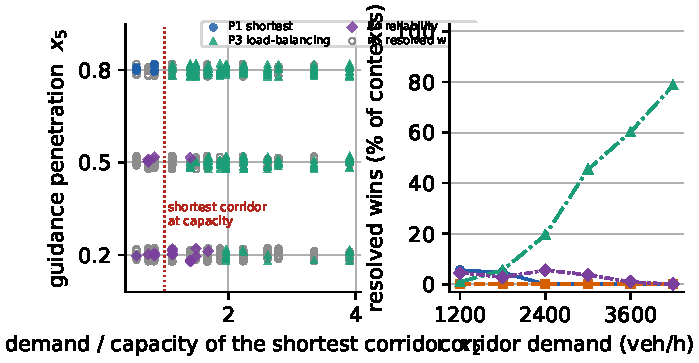
\includegraphics[width=\textwidth]{fig3_regime_map.pdf}
\caption{The regime map. Left: the resolved winner in the plane of shortest-corridor saturation against guidance penetration; open circles mark contexts where the seeds resolve no winner. Right: the share of contexts each policy wins, by demand level.}
\label{fig:regime}
\end{figure}

\begin{table}[t]
\caption{Policy complementarity over 648 contexts. A win is
\emph{resolved} when the paired seed difference against the runner-up exceeds
twice its standard error. Pareto membership is over all three criteria.}
\label{tab:complementarity}
\centering\footnotesize
\setlength{\tabcolsep}{4pt}
\begin{tabular}{@{}l r r r r@{}}
\toprule
& \multicolumn{2}{c}{Best on C1} & \multicolumn{2}{c}{Non-dominated}\\
\cmidrule(lr){2-3}\cmidrule(lr){4-5}
& any & resolved & n & share\\
\midrule
P1 & 21 & 11 & 21 & 3.2\%\\
P2 & 80 & 0 & 266 & 41.0\%\\
P3 & 415 & 227 & 555 & 85.6\%\\
P4 & 132 & 19 & 525 & 81.0\%\\
\midrule
\multicolumn{5}{@{}l}{\emph{Pairwise C1 differences (s/veh); positive = first
policy slower}}\\
\midrule
Pair & mean & 5--95\% range & identical\\
\midrule
P1--P2 & +203.87 & [-0.3, +711.9] & 0.0\%\\
P1--P3 & +220.21 & [+0.8, +761.6] & 0.0\%\\
P1--P4 & +201.87 & [-1.0, +711.9] & 0.0\%\\
P2--P3 & +16.34 & [-0.7, +75.9] & 22.7\%\\
P2--P4 & -2.00 & [-18.2, +9.6] & 42.6\%\\
P3--P4 & -18.34 & [-87.3, +1.3] & 20.2\%\\
\bottomrule
\end{tabular}
\end{table}
\subsection{Decision Value of Adaptation}

Complementarity and decision value are different quantities, and here they point
in opposite directions.

The single-best fixed policy is P3, optimal in 65\%
of contexts. Figure~\ref{fig:performance} shows why the portfolio looks the way
it does: the distance-minimising policy diverges with demand while the three
adaptive policies track one another closely. Running the single-best policy
always costs 474.4~s of system mean journey time per vehicle; the
retrospective per-context best costs 473.9~s. The headroom of
Eq.~\ref{eq:headroom} is therefore
\begin{equation}
H \;=\; 0.451\ \text{s per vehicle},
\qquad
\frac{H}{\mathbb{E}_x[C(x,a_{\mathrm{SBS}})]}
\;=\; \frac{0.451}{474.4} \;=\; 0.095\% .
\end{equation}
This is the aggregate decision headroom relative to the single-best fixed
policy. It is not a claim that any vehicle's travel time improves by
0.095\%; it is the share of the fixed policy's achieved cost that a
perfect per-context choice could remove.

Selecting the wrong \emph{fixed} policy costs far more. Using the
distance-minimising policy throughout increases system mean journey time by
220.2~s per vehicle relative to the single-best fixed policy,
which is 46.4\% of that policy's mean journey time of
474.4~s. The reactive and reliability-aware policies cost
16.3~s (3.4\%) and 18.3~s
(3.9\%) on the same basis.

\begin{quote}
Choosing the fixed policy well is worth 46.4\% of mean journey
time. Choosing it \emph{per context}, given that the best fixed policy is
already in use, is worth 0.095\%.
\end{quote}

The two decisions differ by roughly two and a half orders of magnitude. A
benchmark that reports only the second makes the first invisible, and a system
built to exploit the second while getting the first wrong would be worse than
no system at all.

\begin{figure}[tbp]
\centering
\includegraphics[width=\textwidth]{fig4_performance_pareto.pdf}
\caption{System mean journey time against demand at each guidance penetration level, averaged over the remaining factors. The distance-minimising policy diverges once the shortest corridor saturates, while the three adaptive policies track one another closely --- the visual form of the small decision value quantified in Section~\ref{sec:asymmetry}.}
\label{fig:performance}
\end{figure}

\subsection{Why the Adaptation Headroom Is Small}
\label{sec:asymmetry}

The explanation is not that the policies behave alike; Section~\ref{sec:%
complementarity} shows they do not. It is that the best fixed policy is
near-dominant in a measurable sense.

Define the \emph{downside} of the fixed policy as its mean loss in those
contexts where it is not best, and its \emph{upside} as its mean gain over the
best alternative in those contexts where it is. In 34.3\% of
contexts P3 is not best, and there it loses 1.32~s on
average, at most 17.2~s. In 64.0\% of contexts it is best,
and there it wins by 23.1~s on average, at most 153.5~s.
Its upside is \textbf{18$\times$ its downside}.

A portfolio containing such a member has a large ranking structure and a small
decision structure: any selector moving away from it risks a large loss to
chase a small gain. This is an empirical characterisation of this portfolio in
this environment, not a general theorem. It is, however, measurable in any
portfolio before a selector is built, and we suggest measuring it first.

\subsection{Noise and Statistical Resolution}

Among the 222 contexts where the fixed policy is not best, the
mean headroom is 1.32~s against a mean two-standard-error band
of 1.67~s on the same paired comparison, and the headroom exceeds
its own noise band in 55 of them (25\%).
Resolving the campaign-wide mean effect of 0.451~s under the
criterion of Eq.~\ref{eq:resolved} would require roughly
25 seeds per context, about 64{,}800 runs.

We report this rather than presenting a near-noise-floor improvement as an
achievement. It also bounds what the remaining subsections can claim: selector
differences of a few hundredths of a second per vehicle are real as point
estimates and are not separable from replication noise context by context.

\subsection{Mechanistic Rule}

Fitted on all contexts for exposition, the depth-2 rule splits first on
$x_8 = p\,D/\mathrm{cap}_C$ --- the share of the shortest corridor's
capacity that the guided cohort alone would consume --- at a threshold bracketed
between 0.748 and 0.781. The rule is physically
readable: below that share the decision turns on the effective green ratio;
above it, on whether the arterial is already oversaturated
(Figure~\ref{fig:regions}). This answers RQ2: the preference boundary is
explicable in mechanistic terms, and the explanatory variable is a degree of
saturation rather than a raw demand.

The rule identifies the best policy in 68.8\% of contexts, more often
than always naming the fixed policy does. Its mean decision regret is
nevertheless 0.668~s against 0.451~s for the fixed
policy. \textbf{It is more accurate and more costly.} Under
leave-one-context-out the same pattern holds: B1 reaches 67\% top-1
accuracy against B0's 65\%, and 0.77~s of regret against
0.45~s.

This is the predict-then-optimise distinction~\cite{elmachtoub2022spo} in a
traffic setting. A rule trained to name the winner is rewarded for being right
where the margin is negligible and punished only mildly for being wrong where it
is large --- the wrong trade under an 18$\times$ asymmetry. The
practical implication is that selection accuracy should not be reported as a
proxy for decision quality; in this study the two criteria rank the methods
differently.

\begin{figure}[tbp]
\centering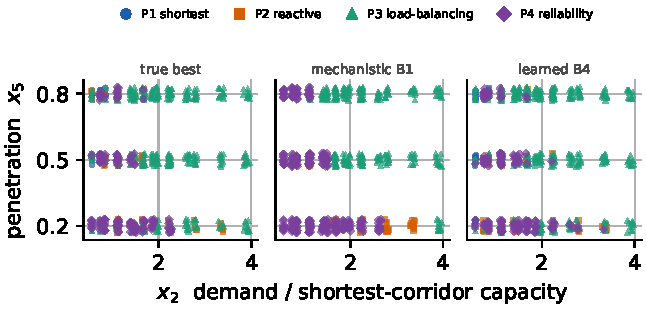
\includegraphics[width=\textwidth]{fig5_selection_regions.pdf}
\caption{Selection regions in the mechanistic feature space: the true best policy, the depth-2 mechanistic rule, and the advantage-based selector, over controlled-flow saturation and guidance penetration.}
\label{fig:regions}
\end{figure}

\subsection{Advantage-Based Selector}

Predicting advantage (Eq.~\ref{eq:advantage}) rather than identity reverses the
failure. B4 reaches 0.20~s of mean regret, closing
55.8\% of the gap between the fixed policy and the retrospective
best, while being \emph{less} accurate at naming the winner (73\%)
than the logistic baseline (76\%, 0.28~s). It also has
the lowest maximum regret of any selector, 7.0~s against
17.2~s (Table~\ref{tab:ladder}, Figure~\ref{fig:ladder}).

The primary comparison declared in advance was B4 against B1. B4 has
substantially lower mean decision regret than B1 (0.20 versus
0.77~s per vehicle). Beating B0 alone would not have been evidence of
much, since B0 is near-dominant by Section~\ref{sec:asymmetry}. This answers
RQ3: a learned selector does identify structure beyond the mechanistic rule ---
but only when trained on the decision cost rather than on the winner's identity.

The magnitude is what matters operationally. B4 reduces mean regret by
0.252~s per vehicle relative to the fixed policy, which is
0.053\% of a 474.4~s mean journey time. The selector is
real and reproducible, and below the threshold at which an operator would act on
it.

\begin{table}[t]
\caption{Decision quality under leave-one-context-out evaluation. Regret is in
seconds of system mean journey time per vehicle. ``Within noise'' is the share
of contexts whose regret falls below that context's own seed noise floor.}
\label{tab:ladder}
\centering\footnotesize
\setlength{\tabcolsep}{3.5pt}
\begin{tabular}{@{}l r r r r r r@{}}
\toprule
& \multicolumn{4}{c}{Regret (s/veh)} & in & gap\\
\cmidrule(lr){2-5}
& mean & med. & max & CVaR$_{90}$ & noise & closed\\
\midrule
B0 ~~best fixed policy & 0.45 & 0.00 & 17.2 & 3.7 & 99\% & ---\\
B1 ~~mechanistic rule & 0.77 & 0.00 & 17.2 & 6.5 & 96\% & -0.714\\
B2 ~~tree, depth 3 & 0.34 & 0.00 & 17.2 & 3.0 & 99\% & 0.238\\
B3 ~~logistic & 0.28 & 0.00 & 17.2 & 2.5 & 100\% & 0.373\\
B4 ~~GBDT advantage & 0.20 & 0.00 & 7.0 & 1.7 & 100\% & 0.558\\
B5 ~~selective, abstaining & 0.45 & 0.00 & 17.2 & 3.7 & 99\% & 0.000\\
~~~VBS (not deployable) & 0.00 & 0.00 & 0.0 & 0.0 & 100\% & 1.000\\
\bottomrule
\end{tabular}
\end{table}
\begin{figure}[tbp]
\centering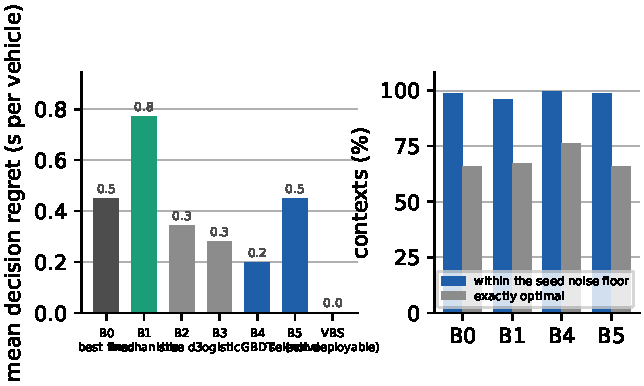
\includegraphics[width=\textwidth]{fig6_decision_ladder.pdf}
\caption{Decision quality under leave-one-context-out evaluation. Left: mean regret for each selector; the hindsight benchmark is hatched because it is not deployable. Right: the share of contexts in which each selector is within the seed noise floor, and exactly optimal.}
\label{fig:ladder}
\end{figure}

\subsection{Selective Prediction and Distribution Shift}

B5 abstains in 36\% of in-distribution contexts and returns exactly
the fixed policy's regret, 0.45~s. The mechanism is explicit rather
than tuned: the conformal interval on the predicted advantage is wider than the
advantage itself, so the requirement that its lower bound exceed zero is never
met. A calibrated gate refuses to act on an effect smaller than its own
uncertainty, which is the correct behaviour given Section~6.5.

Across the 8 shift splits (Table~\ref{tab:ood},
Figure~\ref{fig:ood}) the unguarded selector B4 is \textbf{not uniformly
reliable}. Using a tolerance of 0.05~s per vehicle, it helps on
2 splits, is indistinguishable on 3, and harms on
3:
\begin{itemize}
\item \emph{helps}: the interpolation control O3 (0.56 to
0.17~s) and the domain shift O8 (0.31 to
0.18~s);
\item \emph{indistinguishable}: unseen low demand O2, unseen information lag
O4, unseen penetration O5;
\item \emph{harms}: unseen high demand O1 (0.00 to
0.98~s), unseen green ratio O6, and most severely the concept
shift O7 (0.63 to 2.22~s).
\end{itemize}
Harmful cases therefore occurred under both extrapolation and concept shift,
while two splits improved. \textbf{On each of the 3 harmful splits,
B5 recovered the fixed policy's regret exactly.} The selective rule prevented
the harms that were observed here; it does not guarantee protection against
harms not observed here.

The support gate flags 100\%, 100\% and
100\% of held-out contexts as outside the training envelope
on the lag, penetration and green-ratio extrapolations respectively. The
mechanistic rule degrades worst of all under shift, reaching
6.15~s on unseen penetration, which is consistent with a rule
whose thresholds were fitted inside a range it is now being asked to leave.

\paragraph{A shift the gate cannot see.} O8 is instructive precisely because the
support gate does \emph{not} fire: it flags 0\% of
held-out contexts, because those contexts' descriptors are identical to
descriptors seen in training --- the incident's \emph{location} is not among the
eight. The selector happened to do well there, but it did so unguarded. A
support gate defined on a feature space cannot detect a shift that leaves that
feature space unchanged, and this is a concrete instance rather than a
theoretical caveat. It answers RQ4 with a qualification: abstention removed
every harm we were able to observe, and its coverage is bounded by what the
feature representation can express.

\begin{table}[t]
\caption{Distribution shift, reported separately by shift type. Regret in
seconds of system mean journey time per vehicle on the held-out regime. The
support column is the share of held-out contexts the support gate flagged as
outside the training envelope.}
\label{tab:ood}
\centering\scriptsize
\setlength{\tabcolsep}{3pt}
\begin{tabular}{@{}l l l r r r r r r@{}}
\toprule
& Held out & Shift type & B0 & B1 & B4 & B5 & flagged & abstained\\
\midrule
O1 & demand 4200 & extrapolation & 0.00 & 2.35 & 0.98 & 0.00 & 43\% & 17\%\\
O2 & demand 1200 & extrapolation & 0.53 & 0.52 & 0.53 & 0.53 & 15\% & 75\%\\
O3 & demand 2400 & interpolation & 0.56 & 0.64 & 0.17 & 0.56 & 0\% & 25\%\\
O4 & lag 300 & extrapolation & 0.23 & 0.66 & 0.24 & 0.23 & 100\% & 38\%\\
O5 & penetr. 0.8 & extrapolation & 0.30 & 6.15 & 0.29 & 0.30 & 100\% & 14\%\\
O6 & gc 0.65 & extrapolation & 1.04 & 3.68 & 1.16 & 1.04 & 100\% & 51\%\\
O7 & incident 1 & cov.+concept & 0.63 & 5.33 & 2.22 & 0.63 & 32\% & 36\%\\
O8 & incident on north corr. & domain shift & 0.31 & 0.29 & 0.18 & 0.31 & 0\% & 31\%\\
\bottomrule
\end{tabular}
\end{table}
\begin{figure}[tbp]
\centering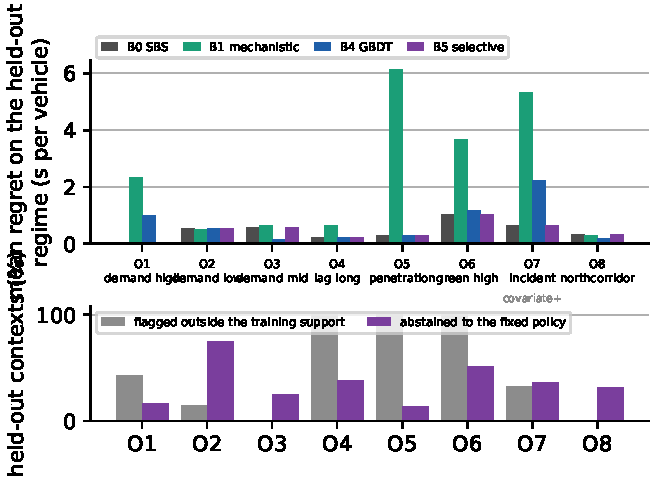
\includegraphics[width=\textwidth]{fig7_ood.pdf}
\caption{Distribution shift, reported separately by shift type. Top: mean regret on the held-out regime for each selector. Bottom: the share of held-out contexts flagged outside the training support, and the share on which the selective selector abstained.}
\label{fig:ood}
\end{figure}

\subsection{Boundary Refinement}
\label{sec:boundary}

13 of the 19 refined sequences are monotone, with a
single change point, and in point estimate they narrow the switching bracket
from the 600~veh/h grid spacing to a median of 150~veh/h.
All 6 shortest-to-load-balancing transitions are monotone; their
change points sit in a 150~veh/h bracket whose position differs by
cell, from 1800--1950~veh/h to
2250--2400~veh/h. That the position moves with
the cell is the point: the boundary is a property of the operating conditions,
not a single number for the network.

\textbf{None of these refined steps is seed-resolved.} The point estimates move
consistently, but no individual step between adjacent refined levels satisfies
Eq.~\ref{eq:resolved} at 5 seeds. The remaining 6
sequences are non-monotone, and all involve the reliability-aware policy. We
therefore report the transition as a point-estimate bracket and state that it is
unresolved: the shortest-path to load-balancing reversal is an ordered regime
change, while the apparent reliability-aware transitions near it are not
distinguishable from noise.

\subsection{Multi-Criteria and Pareto Structure}
\label{sec:pareto}

Over all 648 contexts, 73.0\% have a
non-singleton Pareto set. Non-domination is not concentrated in one policy: P3
is non-dominated in 86\% of contexts, P4 in
81\%, P2 in 41\% and P1 in 3\%.

The criteria are not interchangeable. Journey time and \CO{} correlate at
+0.9390 and rank the four policies identically in
52\% of contexts; journey time and stopped delay correlate at
+0.8916 and agree in only 34\%. The best
policy on \CO{} differs from the best on journey time in
30\% of contexts; on stopped delay it differs in
56\%.

The policies specialise by criterion rather than by regime.
P3 minimises journey time in 418 contexts and
P3 minimises \CO{} in 453, but
\textbf{P4 minimises stopped delay in 429
contexts (66\%)} while minimising journey time in only
129. The reliability-aware policy routes towards the steady,
unsignalised corridor: its vehicles spend less time stationary and more time
moving.

\textbf{This is where the portfolio's complementarity lives} --- on the criterion
vector, not on the scalar cost. An operator whose objective is queue clearance
at signalised junctions and one whose objective is corridor journey time should
not deploy the same policy, and that is a different argmin in
56\% of contexts rather than a preference weighting.

\subsection{Negative Controls and Sensitivity Findings}

\paragraph{Eco-routing is excluded on evidence.} \CO{} and journey time
correlate at +0.9390 and select the same policy in
52\% of contexts. An objective nearly monotone in travel time
adds a label rather than a policy. The numbers are given so a reader may
disagree with the threshold rather than with an assertion.

\paragraph{A policy that never wins.} P2, reactive dynamic travel-time routing,
is never a resolved winner in any of the 648 contexts, and is
non-dominated in only 41\%. In an environment with three
alternatives and an information lag, reacting to the mean is dominated by
balancing load. This is a negative result about a widely deployed policy family
in this environment, and it is reported rather than omitted.

\paragraph{Preference weighting.} Across the three declared preference profiles
the preferred policy changes in 14.5\% of contexts
(Table~\ref{tab:sensitivity}). The journey-time choice is reproduced by the
time-weighted profile in 93\% of contexts, the balanced profile
in 86\% and the environment-weighted profile in
80\%. The decision is stable under reasonable preference
assumptions, and where it is not, stopped delay is what moves it.

\paragraph{Policy parameters.} The dispersion weight of the reliability-aware
policy is close to immaterial, changing that policy's own mean journey time by
at most 0.16\%; across all four parameter changes the identity
of the best policy is unchanged in 78\% to
98\% of the contexts tested. The admissibility tolerance of the
load-balancing policy is not immaterial: loosening it from 0.20 to
0.30 improves that policy's own mean journey time by 2.62\%
(16.7~s). The value fixed in advance therefore \emph{understates} how
dominant the load-balancing policy is, which strengthens rather than weakens the
central conclusion. We report this rather than adopting the better value
retrospectively.

\begin{table}[t]
\caption{Sensitivity and robustness. Upper: the two policy parameters frozen
before the experiment, the effect of changing each on that policy's own mean
journey time, and how often the identity of the best policy is unchanged.
Lower: the three declared preference profiles over normalised criteria, the
policy each selects, and how often that agrees with the journey-time choice.}
\label{tab:sensitivity}
\centering\footnotesize
\setlength{\tabcolsep}{4pt}
\begin{tabular}{@{}l l r r r r r@{}}
\toprule
\multicolumn{7}{@{}l}{\emph{Policy parameters}}\\
\midrule
Policy & Param. & Frozen & Alt. & $\Delta$ (s) & $\Delta$ (\%) & winner same\\
\midrule
P3 & \texttt{p3\_eps} & 0.2 & 0.1 & +8.10 & +1.27\% & 84\%\\
P3 & \texttt{p3\_eps} & 0.2 & 0.3 & -16.66 & -2.62\% & 78\%\\
P4 & \texttt{p4\_lambda} & 1.0 & 0.5 & -0.11 & +0.00\% & 91\%\\
P4 & \texttt{p4\_lambda} & 1.0 & 1.5 & +1.27 & +0.16\% & 98\%\\
\midrule
\multicolumn{7}{@{}l}{\emph{Preference profiles} (weights on normalised C1--C3)}\\
\midrule
Profile & Weights & P1 & P2 & P3 & P4 & agrees C1\\
\midrule
Time & (0.70, 0.15, 0.15) & 19 & 76 & 406 & 147 & 92.9\%\\
Balanced & (0.40, 0.30, 0.30) & 8 & 70 & 399 & 171 & 86.0\%\\
Environment & (0.20, 0.55, 0.25) & 7 & 66 & 425 & 150 & 80.1\%\\
\bottomrule
\end{tabular}
\end{table}
\subsection{Interpretation, Scope, and Limitations}

\paragraph{What the benchmark shows.} Three questions that are usually treated
as one come apart here. The portfolio is complementary; the decision value of
exploiting that complementarity is 0.095\% of the fixed policy's mean
journey time; and a selector capturing that value is not uniformly reliable
outside its training range. The decision carrying substantial value in this
environment is which fixed policy to run --- worth 46.4\% ---
together with which criterion to optimise, since the policy minimising stopped
delay is not the policy minimising journey time in 56\% of
contexts. Both the headroom and its noise floor are computable from paired
replications before any model is built, which we suggest as a standing first
step.

\paragraph{Environment and scope.} The network is synthetic: a controlled
instrument built to isolate mechanisms, not a model of any city. Corridor demand
is a single origin--destination pair choosing among three corridors; the four
minor streets couple the routing decision to traffic that is not routed, but
many simultaneously-routed pairs, with the interactions between their choices,
are outside what is tested. No claim of real-world validation is made anywhere
in this paper. What is portable is the method rather than the numbers: the
descriptors are dimensionless, so a boundary is stated as a degree of saturation
and a controlled-flow share, both measurable on a real network.

\paragraph{Decision context and compliance.} The selector is given the operating
conditions; a deployed system would have to forecast them and would inherit the
forecast's error on top of the selector's. Guided vehicles comply fully, and
unguided vehicles never respond to conditions at all; real behaviour lies
between these. The reported decision quality is therefore an upper bound on what
the same selector would achieve behind a forecast and partial compliance.

\paragraph{Resolution and statistical reach.} The experiment samples a finite
grid with 5 seeds. Boundaries are reported as brackets between
adjacent sampled levels and never as continuous thresholds, and no refined
switching step is seed-resolved (Section~\ref{sec:boundary}). Where a factor is
associated with a change of preferred policy, that is an association within a
designed factorial, not an identified causal mechanism. We report the paired
resolution criterion of Eq.~\ref{eq:resolved} and make no claim of statistical
significance in the hypothesis-testing sense.

\paragraph{Uncertainty machinery.} Split conformal coverage requires
exchangeability, which covariate shift breaks; the conformal gate is calibrated
in-distribution and heuristic outside it, the support gate detects only
extrapolation that is visible in the feature space, and neither detects concept
shift. Split O8 is a demonstrated instance of a shift the support gate does not
see.

\paragraph{Fixed parameters and the emission model.} The policy parameters were
fixed before any evaluation run and are not optima; a looser load-balancing
tolerance improves that policy by 2.62\%, which strengthens the
central conclusion but means the reported value is not the best available.
\CO{} is computed by the simulator's HBEFA3 implementation for one vehicle
class, without fleet composition, cold starts or gradient, so C2 should be read
as a consistent comparative index across policies in this environment rather
than as an absolute emissions estimate. No monetary valuation is used anywhere,
which keeps the study free of invented constants but also means it cannot
express a trade-off in currency.

\section{Conclusion}

We studied context-dependent selection among four established urban routing
policies --- shortest distance, reactive travel time, capacity-aware load
balancing and reliability-aware routing --- in 12{,}960 microsimulation
runs over 648 controlled contexts, with every policy decision taken
from information available before activation and every comparison paired under
common random numbers.

The portfolio is complementary. Three of four policies are strictly best
somewhere by a seed-resolved margin, the winner map depends on more than one
factor, and 73.0\% of contexts have a non-singleton Pareto set
over journey time, \CO{} and stopped delay. The complementarity is strongest on
the criterion vector: the reliability-aware policy minimises stopped delay in
66\% of contexts while rarely minimising journey time.

The decision value of exploiting it is 0.451~s of system mean journey
time per vehicle, 0.095\% of the single-best fixed policy's
474.4~s, because that policy's average gain where it wins is
18$\times$ its average loss where it does not. Selecting the wrong
fixed policy costs 220.2~s per vehicle, 46.4\%
of the same baseline. Within that narrow margin, a selector trained to predict
the winner's identity is more accurate than the fixed policy and more costly
than it, while one trained to predict each policy's advantage has substantially
lower mean decision regret (0.20 versus 0.77~s per
vehicle) and closes 55.8\% of the available gap.

Regime coverage, not model capacity, governs whether that value survives
deployment. Across 8 distribution-shift splits the unguarded
selector helped on 2, was indistinguishable on 3
and harmed on 3, with the largest harm under an unseen disruption
regime. A support-and-confidence gate recovered the fixed policy exactly on
every harmful split, at the cost of the in-distribution gain, and one split
demonstrated a shift the support gate cannot detect because the shift leaves the
feature representation unchanged.

These findings are scoped to the synthetic benchmark described here and are not
evidence about any real network. Within that scope, the benchmark separates
three questions usually treated as one --- whether policies are complementary,
whether adaptation carries decision value, and whether a selector can be
deployed safely --- and shows that the answers can differ. The most useful next
step is to repeat the measurement where several origin--destination pairs are
routed simultaneously, since the interaction between their choices is the
mechanism most likely to change the size of the headroom.


\bibliographystyle{splncs04}
\bibliography{references}

\end{document}
